\chapter{Anexo}

\section{Análisis de errores extremos: detalle por barra}
\label{anexo:errores_extremos}

Esta sección presenta el detalle completo del análisis de errores extremos introducido en la Sección \ref{sec:errores_extremos}, para las siete barras del SEN no mostradas allí (Atacama se presenta en el cuerpo principal como caso ilustrativo, incluyendo su distribución de errores; las ocho barras exhiben la misma forma general, por lo que aquí no se repite la figura de distribución). Para cada barra se incluye la tabla de los 20 mayores errores con su clasificación (\textit{desfase de fase} vs.\ \textit{evento estructural}, según el criterio de desplazamiento descrito en la Sección \ref{sec:errores_extremos}) y un panel con cuatro casos representativos. La Tabla \ref{tab:sintesis_errores} resume los resultados agregados de las ocho barras, incluyendo el MAE, el percentil 95 y el máximo de cada una.

\subsection{Cardones}

\begin{table}[htbp]
    \centering
    \small
    \begin{tabular}{rllrr}
        \toprule
        Rank & Fecha       & Hora  & Error abs.\ (USD/MWh) & Tipo \\
        \midrule
 1 & 2024-08-31 & 23:00 & 164.48 & Desfase de fase \\
 2 & 2024-08-09 & 08:00 & 147.34 & Evento estructural \\
 3 & 2024-11-25 & 07:00 & 126.22 & Evento estructural \\
 4 & 2025-02-11 & 05:00 & 117.56 & Desfase de fase \\
 5 & 2025-02-11 & 02:00 & 117.19 & Desfase de fase \\
 6 & 2025-03-25 & 07:00 & 113.85 & Desfase de fase \\
 7 & 2024-09-04 & 19:00 & 111.95 & Desfase de fase \\
 8 & 2024-10-03 & 21:00 & 111.70 & Desfase de fase \\
 9 & 2025-04-10 & 07:00 & 111.15 & Desfase de fase \\
10 & 2025-03-25 & 20:00 & 104.93 & Desfase de fase \\
11 & 2025-04-06 & 07:00 & 102.11 & Evento estructural \\
12 & 2024-09-04 & 20:00 & 101.22 & Desfase de fase \\
13 & 2025-02-26 & 05:00 & 100.97 & Desfase de fase \\
14 & 2024-10-04 & 07:00 & 100.63 & Desfase de fase \\
15 & 2025-04-19 & 21:00 &  98.16 & Desfase de fase \\
16 & 2025-02-26 & 23:00 &  97.61 & Desfase de fase \\
17 & 2024-09-27 & 00:00 &  95.43 & Desfase de fase \\
18 & 2025-01-27 & 04:00 &  91.98 & Desfase de fase \\
19 & 2025-04-21 & 01:00 &  90.53 & Desfase de fase \\
20 & 2024-11-08 & 23:00 &  90.21 & Desfase de fase \\
        \bottomrule
    \end{tabular}
    \vspace{0.2cm}
    \caption{Los 20 mayores errores absolutos del $\text{TFT}_\text{LN}$ (S+C) en validación, Cardones.}
    \label{tab:top20_cardones}
\end{table}

\begin{figure}[htbp]
    \centering
    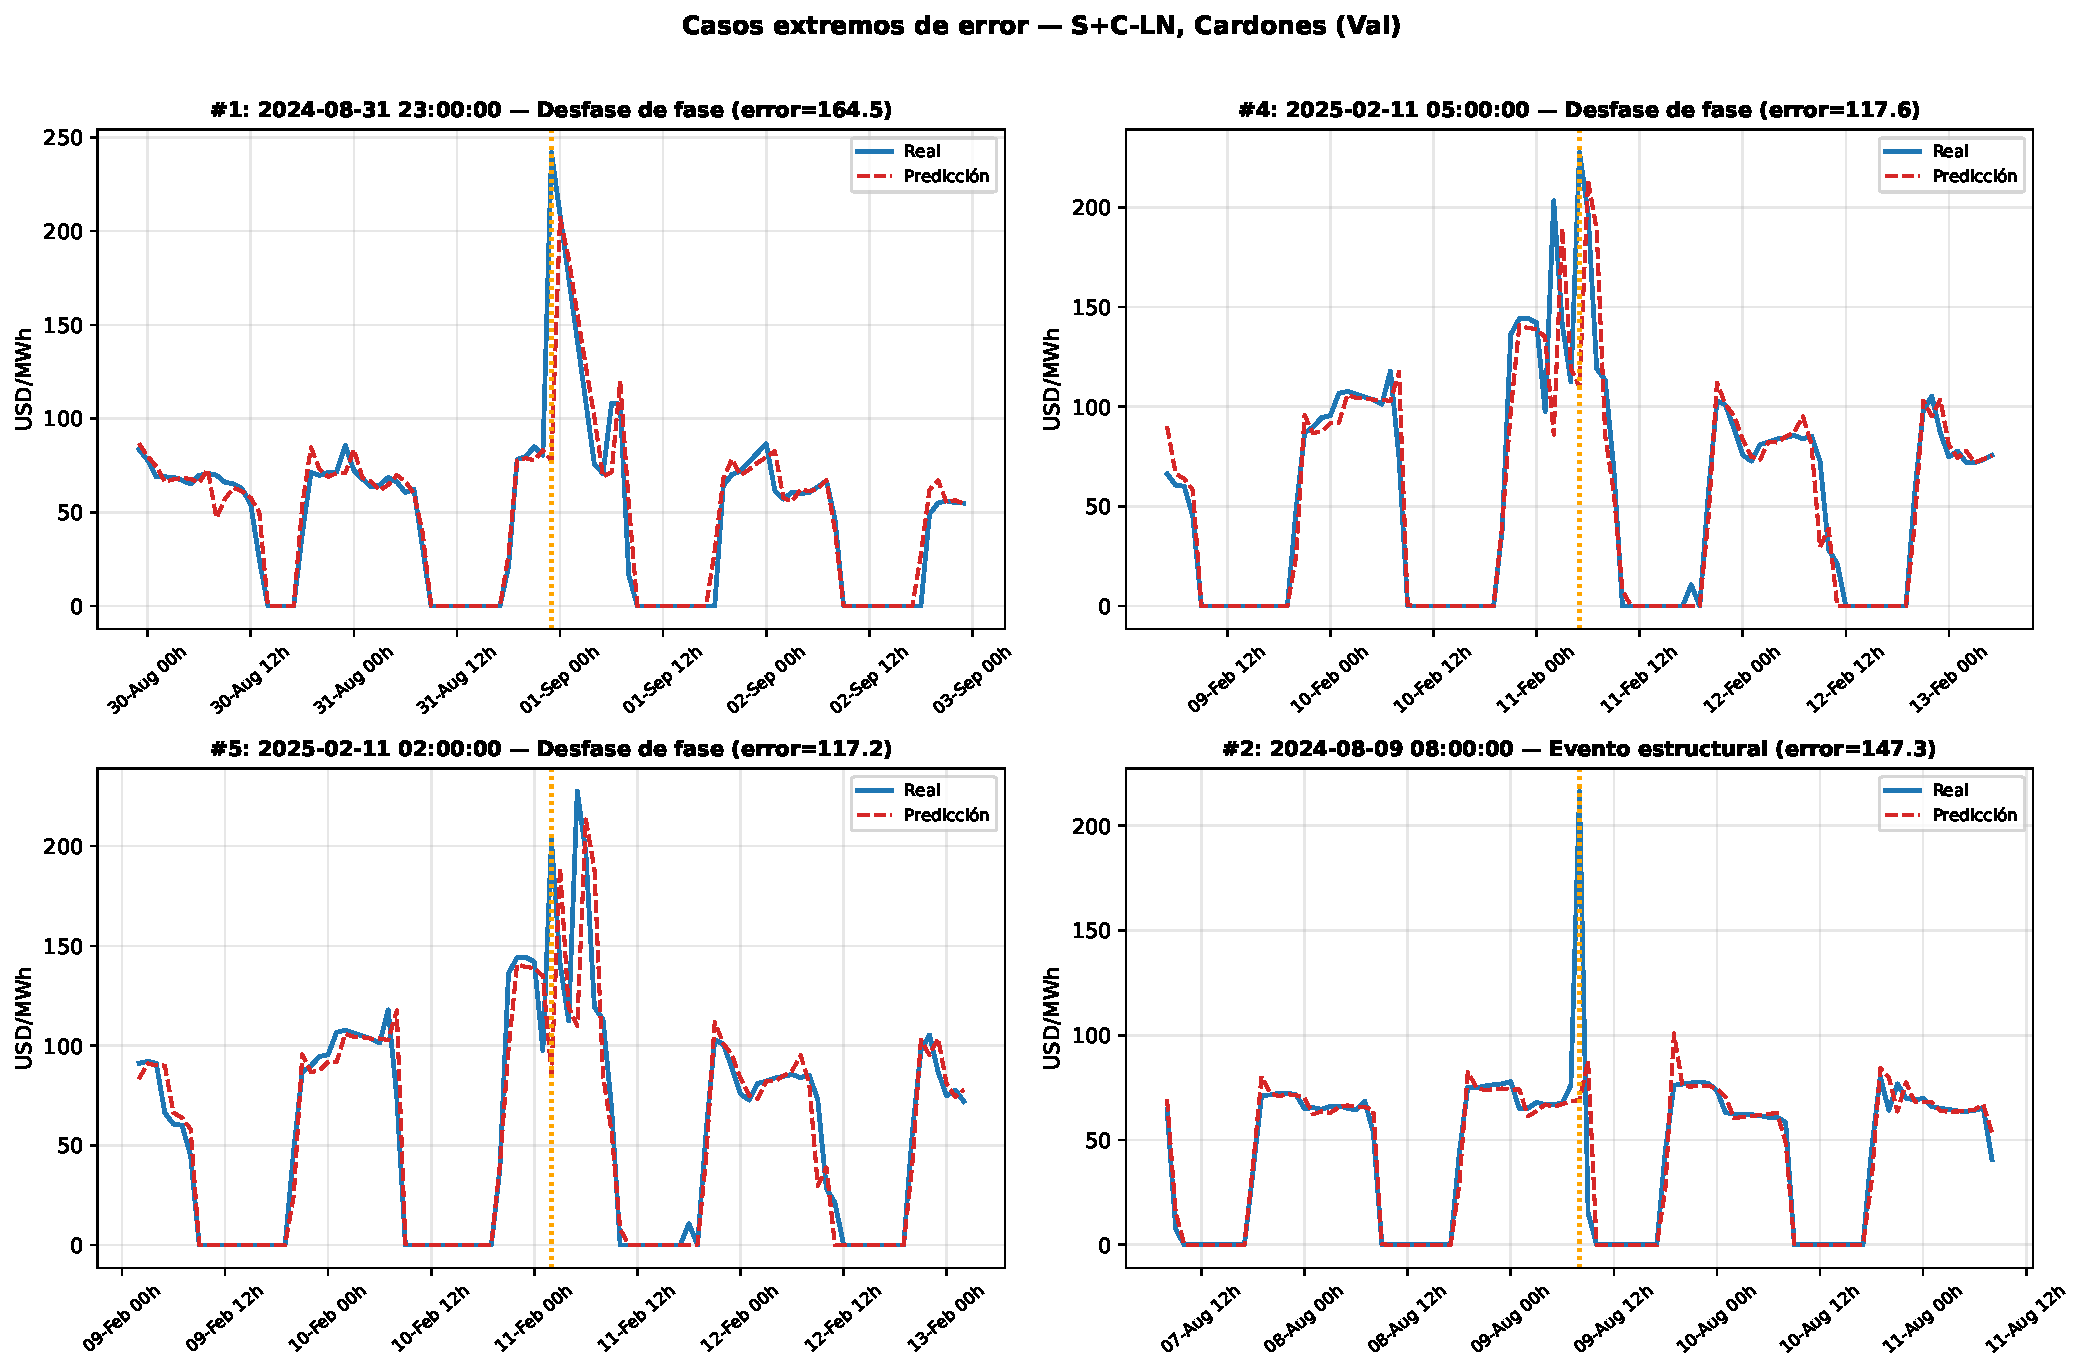
\includegraphics[width=\textwidth]{imagenes/fig_phase_shift_panel_cardones.pdf}
    \caption{Casos extremos de error del $\text{TFT}_\text{LN}$ (S+C), Cardones.}
    \label{fig:phase_shift_panel_cardones}
\end{figure}

\clearpage
\subsection{Charrúa}

\begin{table}[htbp]
    \centering
    \small
    \begin{tabular}{rllrr}
        \toprule
        Rank & Fecha       & Hora  & Error abs.\ (USD/MWh) & Tipo \\
        \midrule
 1 & 2024-08-09 & 08:00 & 132.36 & Desfase de fase \\
 2 & 2024-08-09 & 09:00 & 128.18 & Desfase de fase \\
 3 & 2025-04-01 & 20:00 & 115.24 & Desfase de fase \\
 4 & 2025-02-28 & 10:00 & 114.44 & Desfase de fase \\
 5 & 2025-03-25 & 13:00 & 107.90 & Desfase de fase \\
 6 & 2025-02-26 & 05:00 & 106.61 & Desfase de fase \\
 7 & 2025-03-26 & 09:00 & 105.77 & Evento estructural \\
 8 & 2024-11-25 & 07:00 & 105.55 & Evento estructural \\
 9 & 2025-03-25 & 07:00 & 104.93 & Desfase de fase \\
10 & 2025-04-10 & 07:00 & 100.32 & Desfase de fase \\
11 & 2025-02-11 & 02:00 &  98.89 & Desfase de fase \\
12 & 2025-02-11 & 05:00 &  95.81 & Desfase de fase \\
13 & 2025-04-21 & 01:00 &  95.41 & Desfase de fase \\
14 & 2025-04-06 & 07:00 &  95.32 & Evento estructural \\
15 & 2025-03-27 & 10:00 &  93.44 & Desfase de fase \\
16 & 2025-04-08 & 16:00 &  92.60 & Desfase de fase \\
17 & 2024-06-22 & 18:00 &  92.51 & Desfase de fase \\
18 & 2024-10-03 & 21:00 &  92.20 & Desfase de fase \\
19 & 2025-03-24 & 20:00 &  92.10 & Desfase de fase \\
20 & 2025-04-11 & 08:00 &  91.56 & Desfase de fase \\
        \bottomrule
    \end{tabular}
    \vspace{0.2cm}
    \caption{Los 20 mayores errores absolutos del $\text{TFT}_\text{LN}$ (S+C) en validación, Charrúa.}
    \label{tab:top20_charrua}
\end{table}

\begin{figure}[htbp]
    \centering
    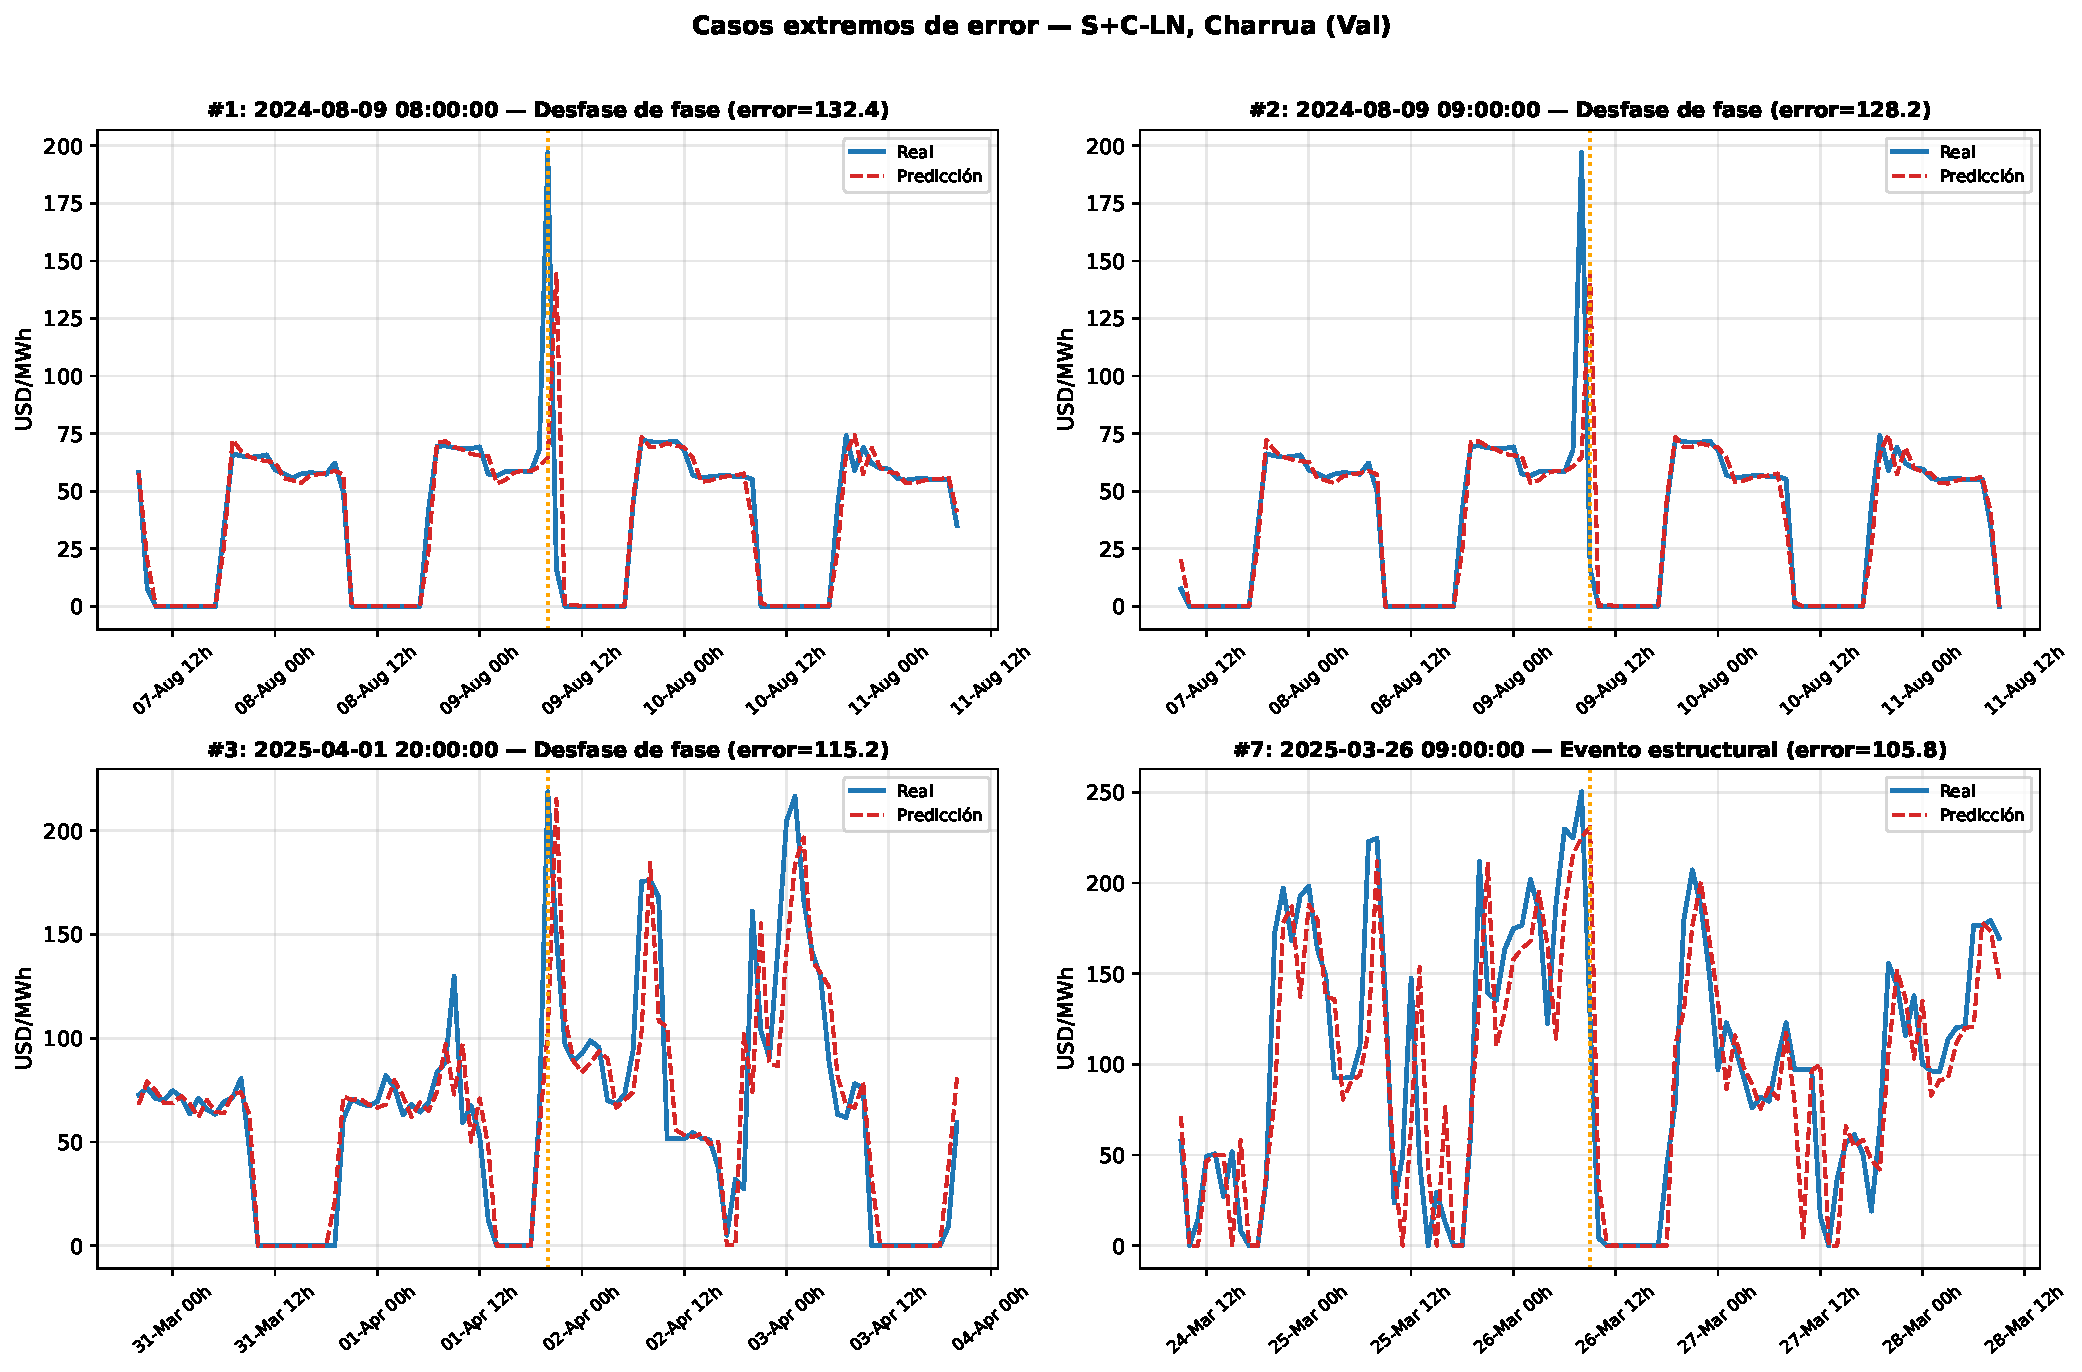
\includegraphics[width=\textwidth]{imagenes/fig_phase_shift_panel_charrua.pdf}
    \caption{Casos extremos de error del $\text{TFT}_\text{LN}$ (S+C), Charrúa.}
    \label{fig:phase_shift_panel_charrua}
\end{figure}

\clearpage
\subsection{Crucero}

\begin{table}[htbp]
    \centering
    \small
    \begin{tabular}{rllrr}
        \toprule
        Rank & Fecha       & Hora  & Error abs.\ (USD/MWh) & Tipo \\
        \midrule
 1 & 2024-08-31 & 23:00 & 174.38 & Desfase de fase \\
 2 & 2024-09-03 & 21:00 & 155.89 & Desfase de fase \\
 3 & 2024-08-09 & 08:00 & 152.69 & Evento estructural \\
 4 & 2024-11-25 & 07:00 & 136.43 & Evento estructural \\
 5 & 2025-02-11 & 02:00 & 128.65 & Desfase de fase \\
 6 & 2025-02-11 & 05:00 & 126.79 & Desfase de fase \\
 7 & 2024-09-04 & 19:00 & 122.14 & Desfase de fase \\
 8 & 2024-09-04 & 03:00 & 115.40 & Desfase de fase \\
 9 & 2025-03-25 & 07:00 & 114.71 & Desfase de fase \\
10 & 2024-10-03 & 21:00 & 113.51 & Desfase de fase \\
11 & 2024-10-04 & 07:00 & 110.96 & Desfase de fase \\
12 & 2025-04-01 & 20:00 & 107.42 & Desfase de fase \\
13 & 2025-04-10 & 07:00 & 104.85 & Desfase de fase \\
14 & 2025-04-21 & 20:00 & 104.33 & Desfase de fase \\
15 & 2024-11-08 & 23:00 & 103.60 & Desfase de fase \\
16 & 2025-04-19 & 21:00 & 101.84 & Desfase de fase \\
17 & 2025-05-05 & 19:00 &  99.22 & Desfase de fase \\
18 & 2024-09-27 & 00:00 &  98.65 & Desfase de fase \\
19 & 2024-10-04 & 00:00 &  98.04 & Desfase de fase \\
20 & 2025-03-25 & 20:00 &  97.99 & Desfase de fase \\
        \bottomrule
    \end{tabular}
    \vspace{0.2cm}
    \caption{Los 20 mayores errores absolutos del $\text{TFT}_\text{LN}$ (S+C) en validación, Crucero.}
    \label{tab:top20_crucero}
\end{table}

\begin{figure}[htbp]
    \centering
    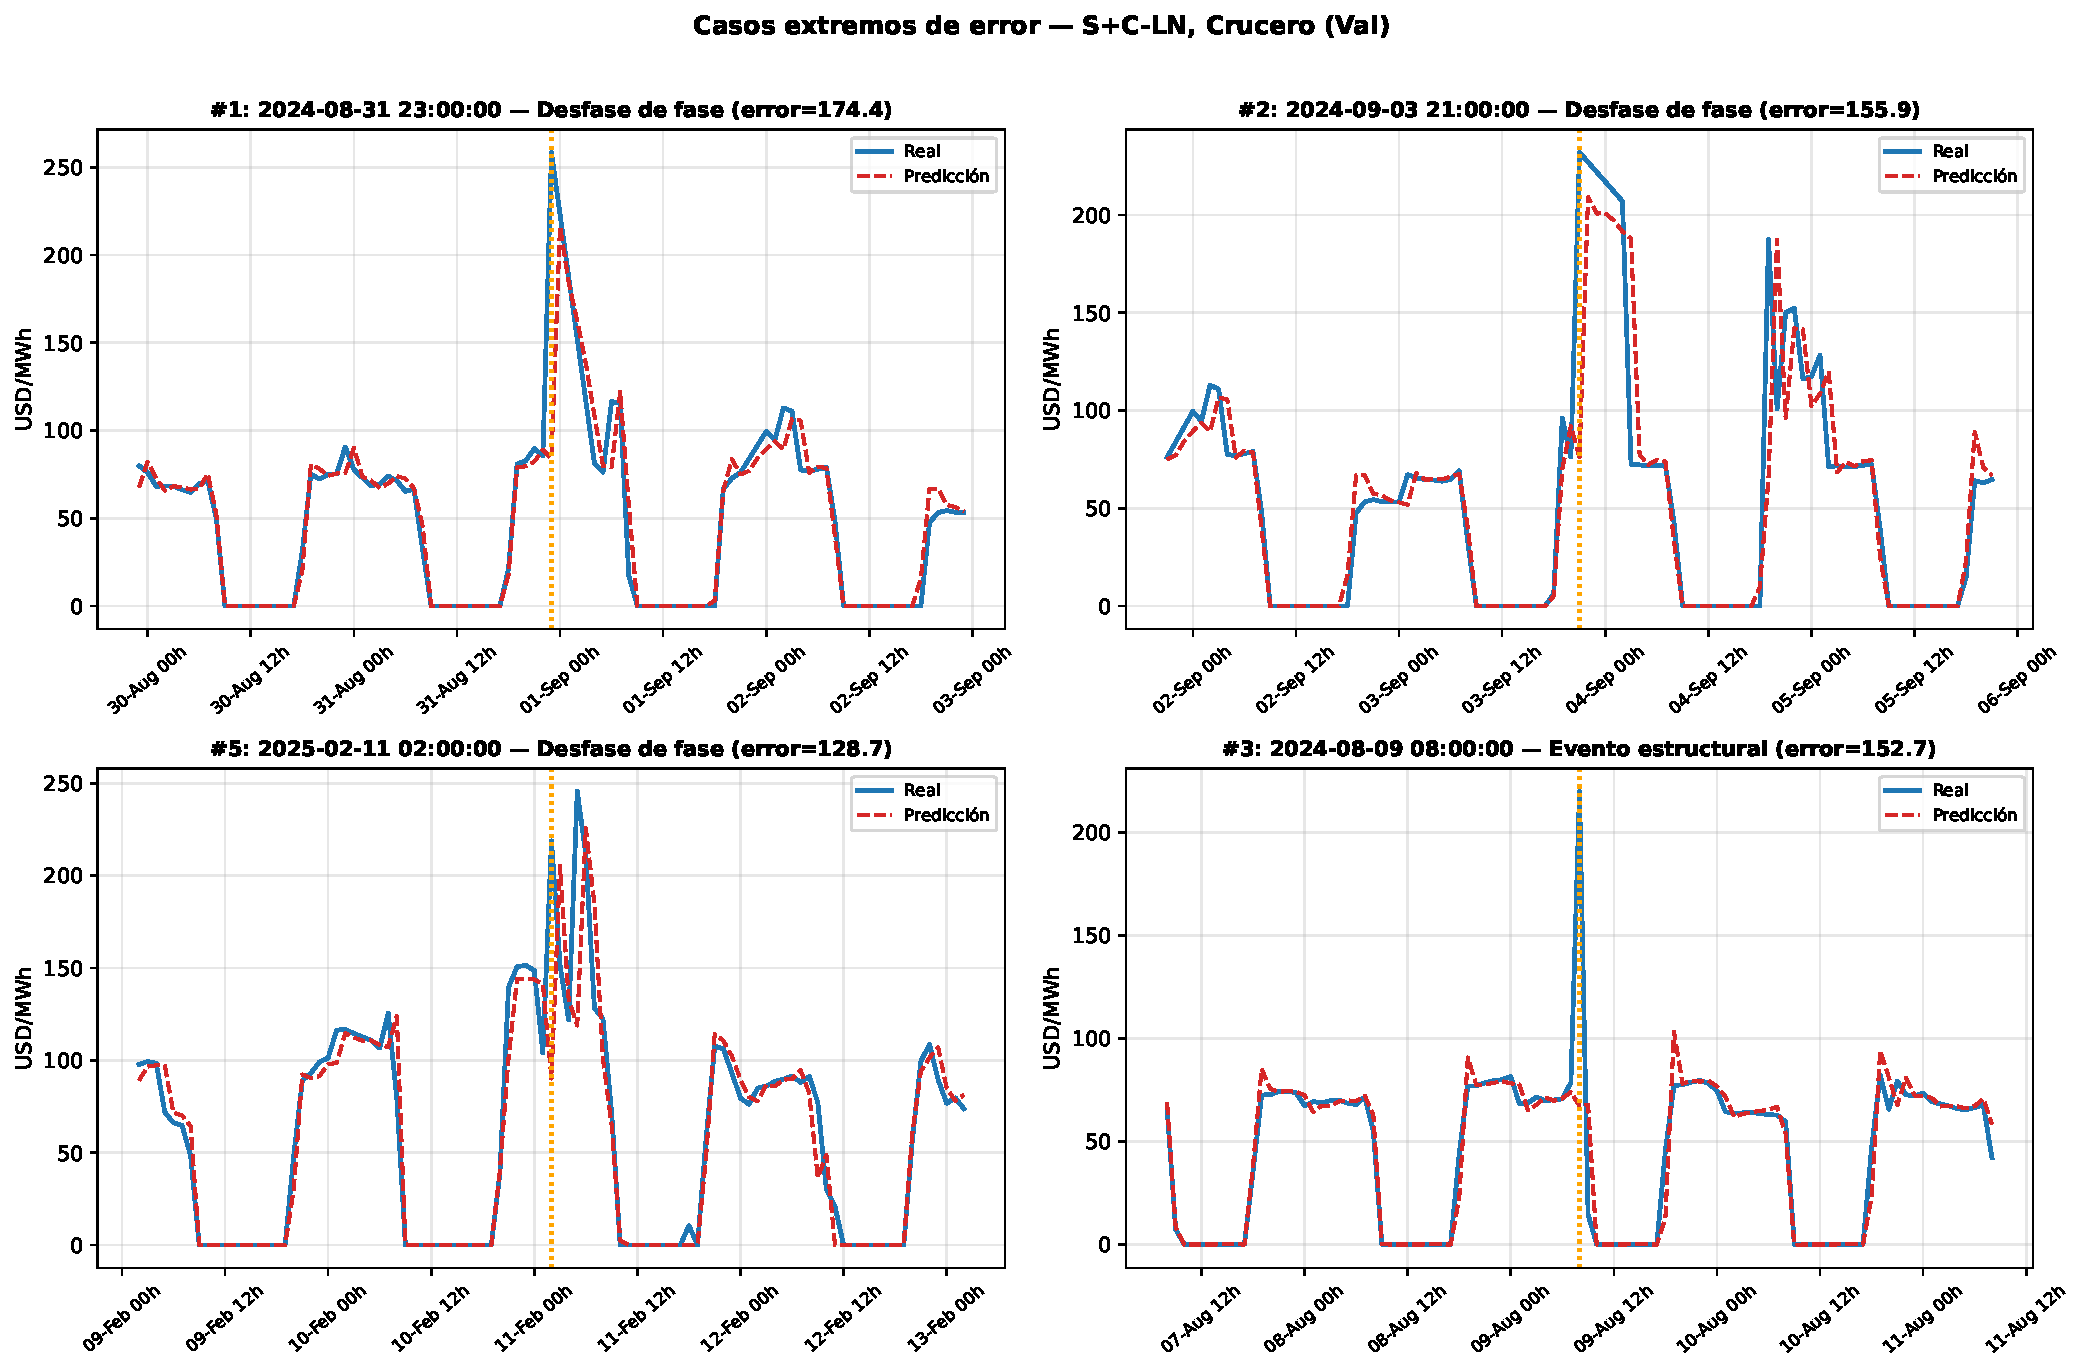
\includegraphics[width=\textwidth]{imagenes/fig_phase_shift_panel_crucero.pdf}
    \caption{Casos extremos de error del $\text{TFT}_\text{LN}$ (S+C), Crucero.}
    \label{fig:phase_shift_panel_crucero}
\end{figure}

\clearpage
\subsection{Pan de Azúcar}

\begin{table}[htbp]
    \centering
    \small
    \begin{tabular}{rllrr}
        \toprule
        Rank & Fecha       & Hora  & Error abs.\ (USD/MWh) & Tipo \\
        \midrule
 1 & 2024-08-09 & 08:00 & 143.70 & Evento estructural \\
 2 & 2025-04-09 & 10:00 & 141.93 & Desfase de fase \\
 3 & 2024-11-25 & 07:00 & 121.17 & Evento estructural \\
 4 & 2025-02-11 & 05:00 & 116.00 & Desfase de fase \\
 5 & 2025-02-28 & 10:00 & 114.26 & Desfase de fase \\
 6 & 2025-03-25 & 07:00 & 114.06 & Desfase de fase \\
 7 & 2025-04-10 & 07:00 & 113.39 & Desfase de fase \\
 8 & 2025-02-11 & 02:00 & 112.29 & Desfase de fase \\
 9 & 2024-10-03 & 21:00 & 108.08 & Desfase de fase \\
10 & 2025-04-01 & 20:00 & 102.58 & Desfase de fase \\
11 & 2025-04-19 & 21:00 & 101.46 & Desfase de fase \\
12 & 2024-10-09 & 09:00 &  99.98 & Desfase de fase \\
13 & 2025-03-25 & 20:00 &  98.47 & Desfase de fase \\
14 & 2025-04-08 & 16:00 &  97.98 & Desfase de fase \\
15 & 2025-02-26 & 05:00 &  97.62 & Desfase de fase \\
16 & 2025-04-06 & 07:00 &  95.02 & Evento estructural \\
17 & 2024-11-08 & 23:00 &  94.82 & Desfase de fase \\
18 & 2024-09-27 & 00:00 &  93.71 & Desfase de fase \\
19 & 2024-10-04 & 07:00 &  91.10 & Desfase de fase \\
20 & 2025-04-21 & 01:00 &  90.23 & Desfase de fase \\
        \bottomrule
    \end{tabular}
    \vspace{0.2cm}
    \caption{Los 20 mayores errores absolutos del $\text{TFT}_\text{LN}$ (S+C) en validación, Pan de Azúcar.}
    \label{tab:top20_pazucar}
\end{table}

\begin{figure}[htbp]
    \centering
    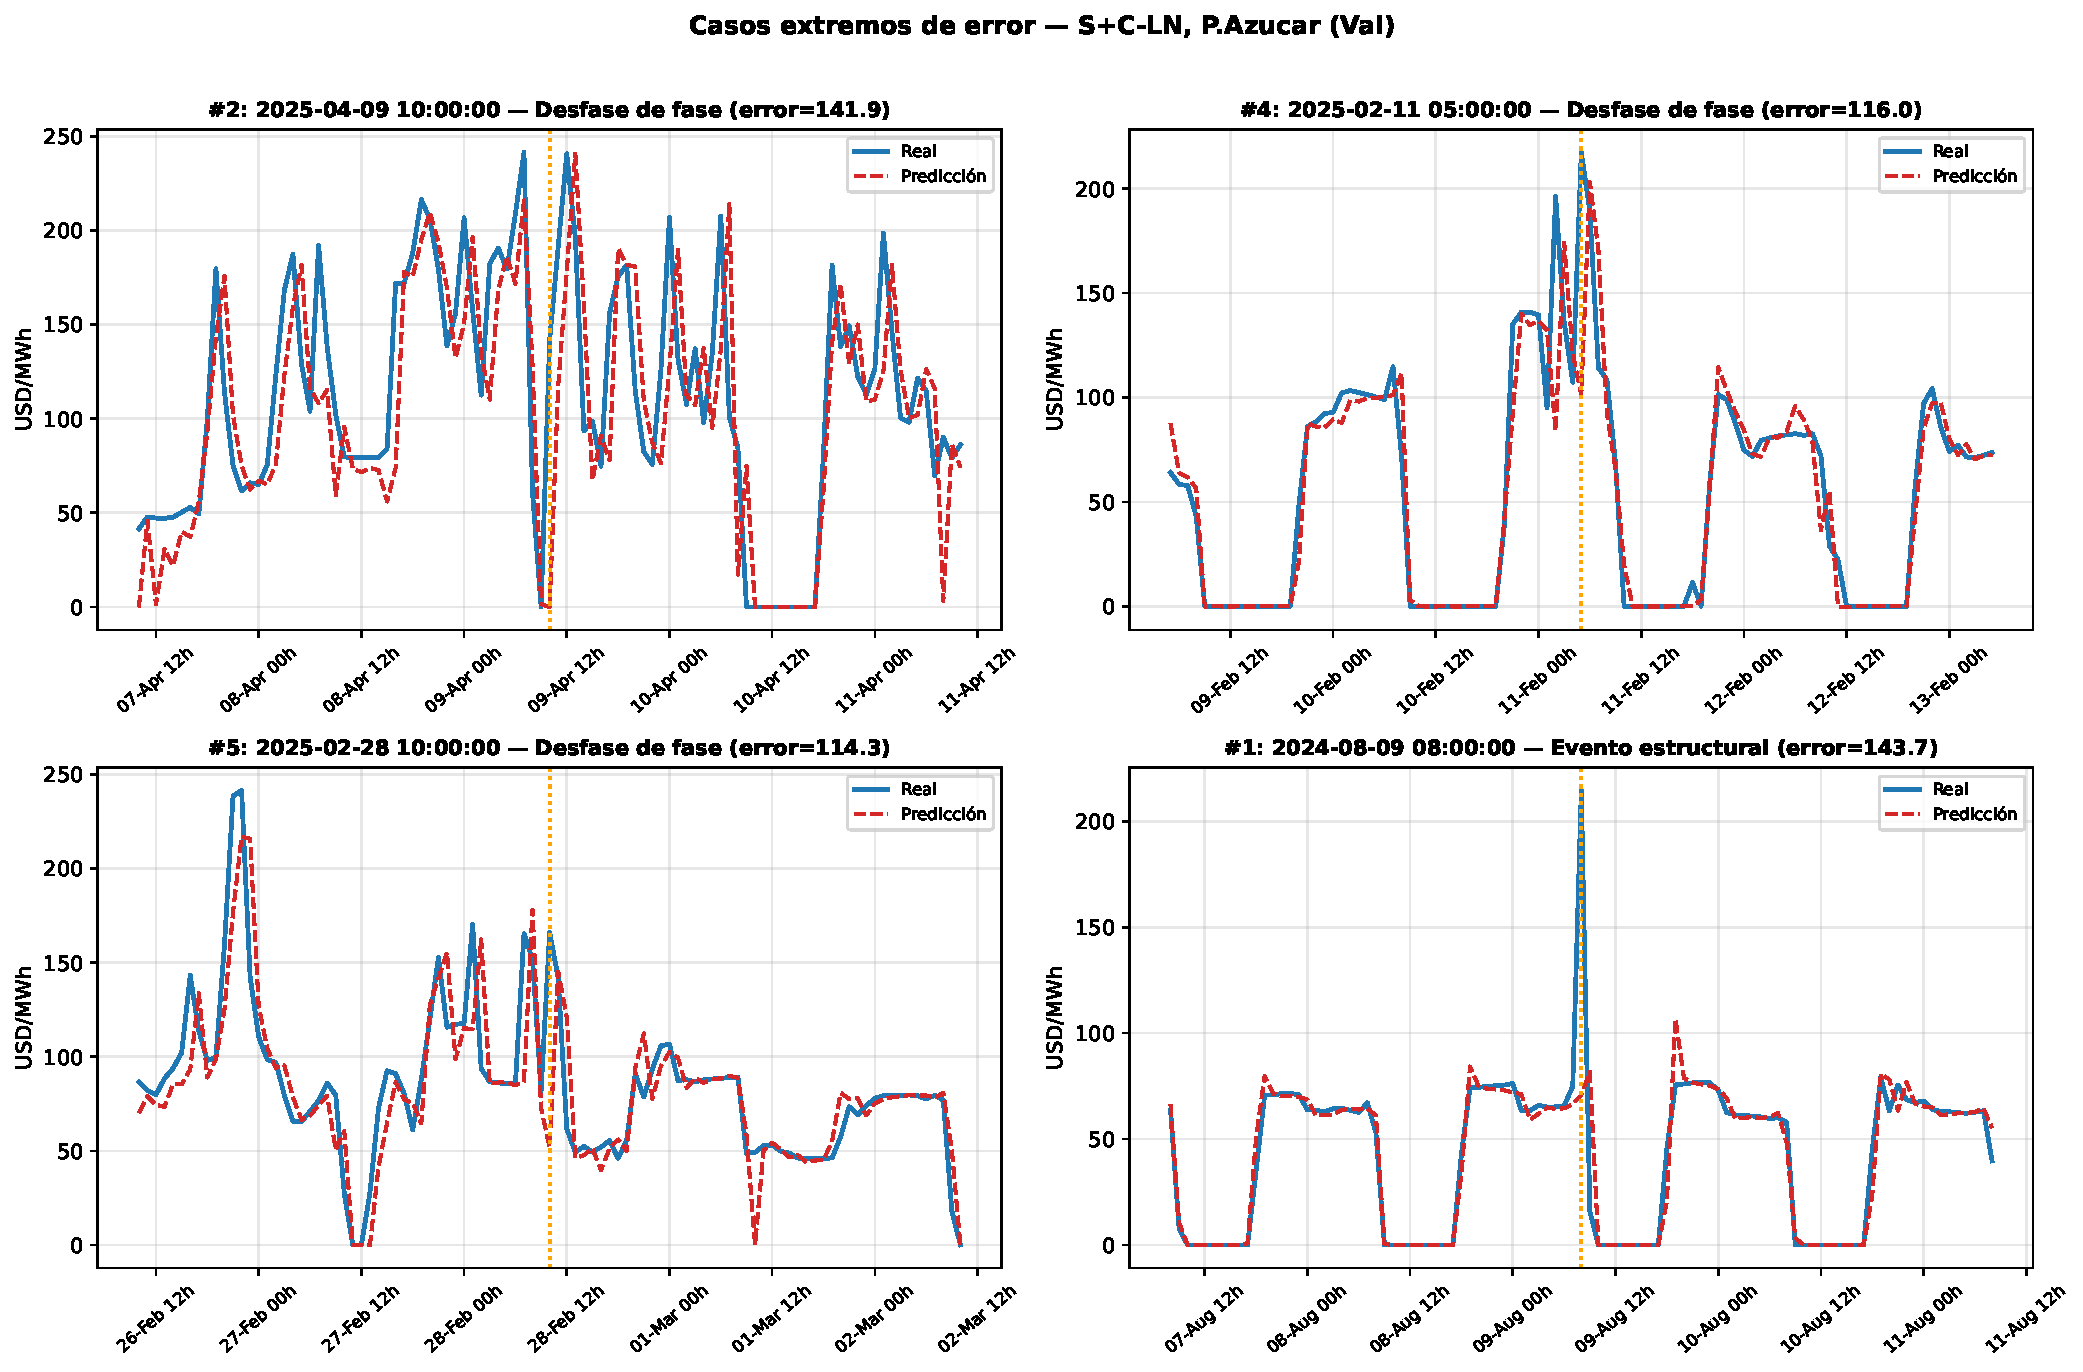
\includegraphics[width=\textwidth]{imagenes/fig_phase_shift_panel_pazucar.pdf}
    \caption{Casos extremos de error del $\text{TFT}_\text{LN}$ (S+C), Pan de Azúcar.}
    \label{fig:phase_shift_panel_pazucar}
\end{figure}

\clearpage
\subsection{Puerto Montt}

\begin{table}[htbp]
    \centering
    \small
    \begin{tabular}{rllrr}
        \toprule
        Rank & Fecha       & Hora  & Error abs.\ (USD/MWh) & Tipo \\
        \midrule
 1 & 2024-08-08 & 10:00 & 241.73 & Desfase de fase \\
 2 & 2025-01-31 & 09:00 & 230.86 & Desfase de fase \\
 3 & 2025-02-01 & 10:00 & 221.28 & Desfase de fase \\
 4 & 2025-02-17 & 10:00 & 218.87 & Desfase de fase \\
 5 & 2024-07-27 & 10:00 & 215.08 & Desfase de fase \\
 6 & 2024-07-21 & 01:00 & 211.68 & Desfase de fase \\
 7 & 2024-08-07 & 11:00 & 207.02 & Desfase de fase \\
 8 & 2025-02-09 & 12:00 & 205.38 & Desfase de fase \\
 9 & 2025-02-14 & 20:00 & 198.06 & Desfase de fase \\
10 & 2025-02-08 & 05:00 & 196.61 & Desfase de fase \\
11 & 2025-01-09 & 11:00 & 195.40 & Desfase de fase \\
12 & 2024-07-22 & 12:00 & 191.37 & Desfase de fase \\
13 & 2025-02-16 & 12:00 & 190.55 & Desfase de fase \\
14 & 2025-01-30 & 18:00 & 188.20 & Desfase de fase \\
15 & 2024-07-29 & 16:00 & 188.11 & Desfase de fase \\
16 & 2025-01-12 & 16:00 & 183.57 & Desfase de fase \\
17 & 2024-07-21 & 02:00 & 183.27 & Desfase de fase \\
18 & 2025-02-09 & 11:00 & 183.13 & Desfase de fase \\
19 & 2024-07-30 & 13:00 & 182.82 & Desfase de fase \\
20 & 2024-07-29 & 11:00 & 182.36 & Desfase de fase \\
        \bottomrule
    \end{tabular}
    \vspace{0.2cm}
    \caption{Los 20 mayores errores absolutos del $\text{TFT}_\text{LN}$ (S+C) en validación, Puerto Montt. A diferencia del resto de las barras, ninguno cae en horas de transición solar (07:00--08:00, 19:00--21:00) ni comparte fecha con los eventos de las demás barras, consistente con una dinámica gobernada por la disponibilidad hidroeléctrica.}
    \label{tab:top20_pmontt}
\end{table}

\begin{figure}[htbp]
    \centering
    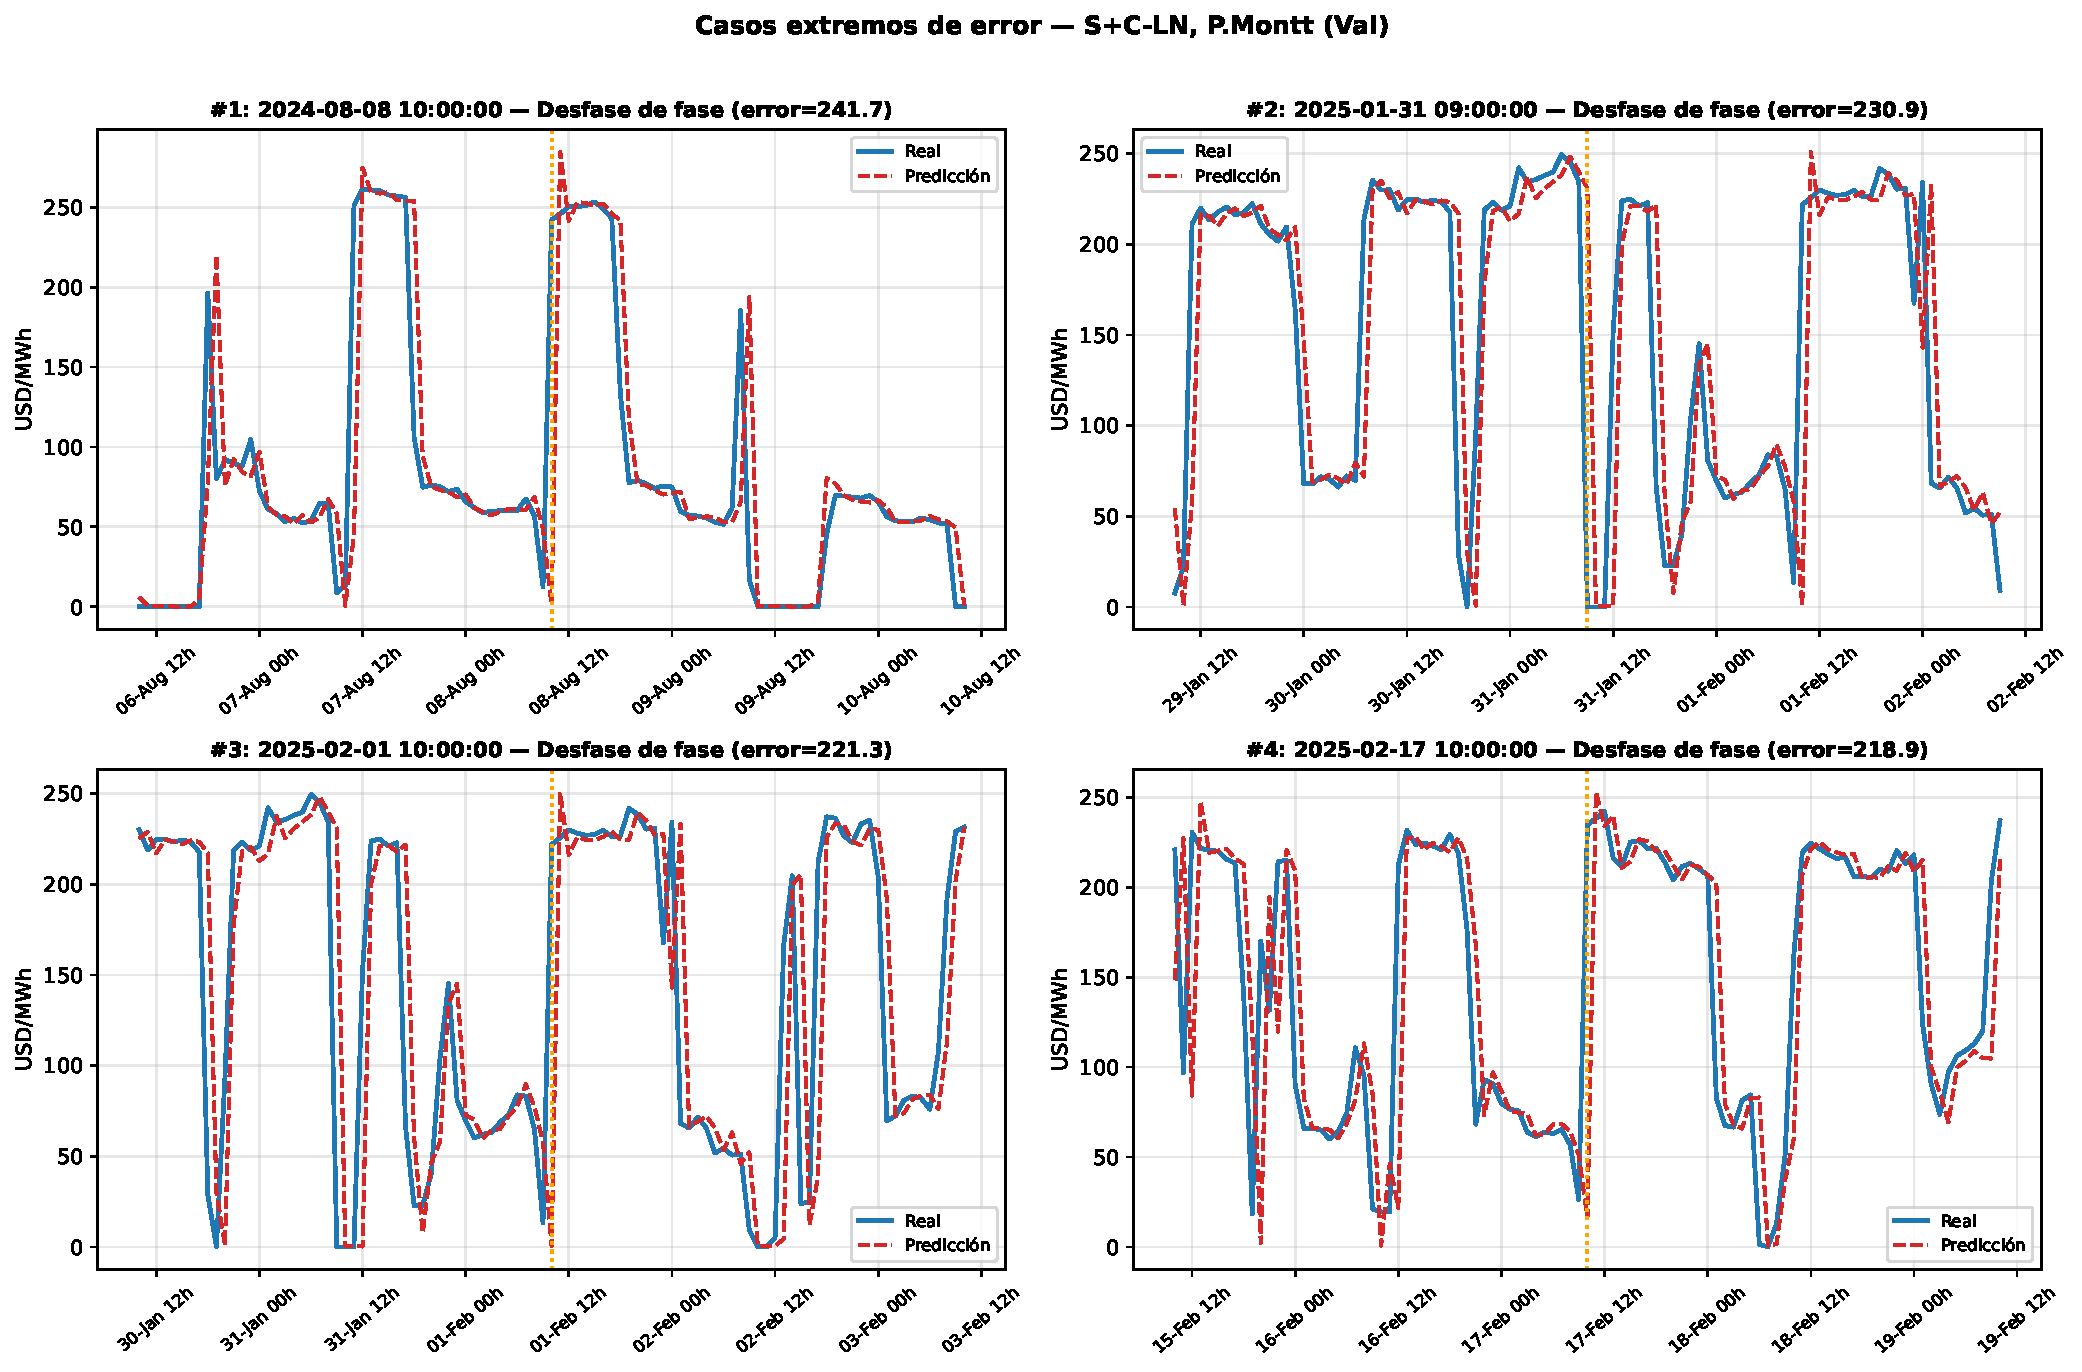
\includegraphics[width=\textwidth]{imagenes/fig_phase_shift_panel_pmontt.pdf}
    \caption{Casos extremos de error del $\text{TFT}_\text{LN}$ (S+C), Puerto Montt.}
    \label{fig:phase_shift_panel_pmontt}
\end{figure}

\clearpage
\subsection{Quillota}

\begin{table}[htbp]
    \centering
    \small
    \begin{tabular}{rllrr}
        \toprule
        Rank & Fecha       & Hora  & Error abs.\ (USD/MWh) & Tipo \\
        \midrule
 1 & 2024-08-09 & 08:00 & 144.20 & Evento estructural \\
 2 & 2025-04-01 & 20:00 & 136.59 & Desfase de fase \\
 3 & 2025-04-10 & 07:00 & 133.54 & Desfase de fase \\
 4 & 2025-04-09 & 09:00 & 122.63 & Desfase de fase \\
 5 & 2025-02-28 & 10:00 & 115.66 & Desfase de fase \\
 6 & 2024-11-25 & 07:00 & 113.03 & Evento estructural \\
 7 & 2025-03-25 & 07:00 & 110.41 & Desfase de fase \\
 8 & 2024-10-03 & 21:00 & 105.31 & Desfase de fase \\
 9 & 2025-02-11 & 05:00 & 105.15 & Desfase de fase \\
10 & 2025-04-06 & 07:00 & 104.96 & Evento estructural \\
11 & 2025-02-26 & 05:00 & 102.50 & Desfase de fase \\
12 & 2025-02-11 & 02:00 & 101.02 & Desfase de fase \\
13 & 2025-04-21 & 01:00 &  95.57 & Desfase de fase \\
14 & 2024-06-22 & 18:00 &  95.36 & Desfase de fase \\
15 & 2024-06-17 & 23:00 &  92.82 & Evento estructural \\
16 & 2025-04-11 & 08:00 &  92.05 & Desfase de fase \\
17 & 2024-11-08 & 23:00 &  91.39 & Desfase de fase \\
18 & 2025-03-25 & 13:00 &  91.01 & Desfase de fase \\
19 & 2025-03-27 & 10:00 &  90.81 & Desfase de fase \\
20 & 2025-04-08 & 16:00 &  90.71 & Desfase de fase \\
        \bottomrule
    \end{tabular}
    \vspace{0.2cm}
    \caption{Los 20 mayores errores absolutos del $\text{TFT}_\text{LN}$ (S+C) en validación, Quillota.}
    \label{tab:top20_quillota}
\end{table}

\begin{figure}[htbp]
    \centering
    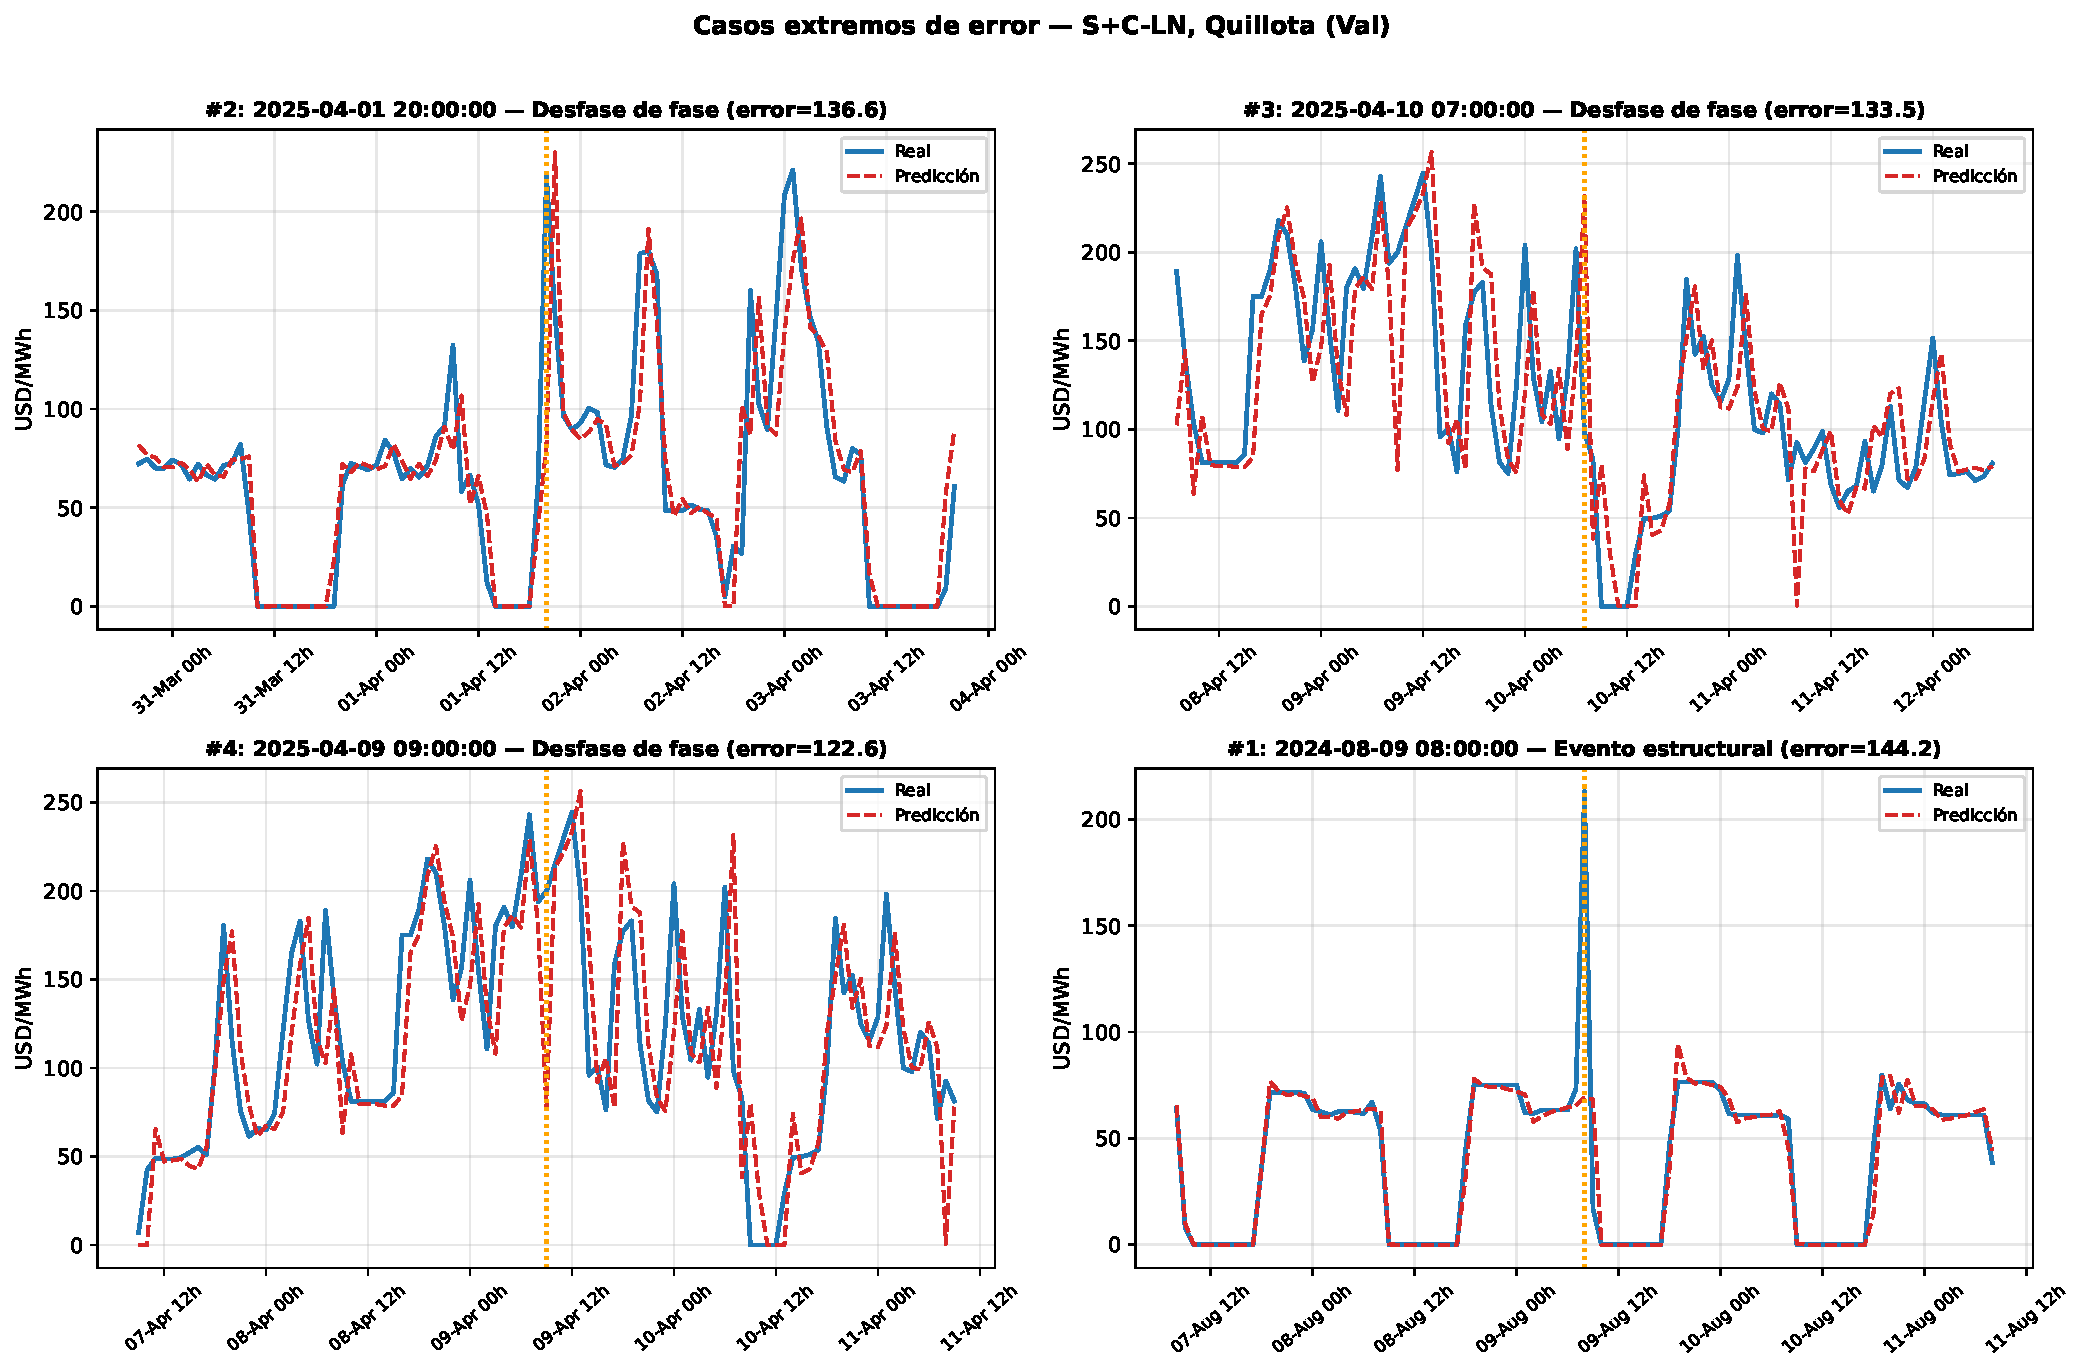
\includegraphics[width=\textwidth]{imagenes/fig_phase_shift_panel_quillota.pdf}
    \caption{Casos extremos de error del $\text{TFT}_\text{LN}$ (S+C), Quillota.}
    \label{fig:phase_shift_panel_quillota}
\end{figure}

\clearpage
\subsection{Tarapacá}

\begin{table}[htbp]
    \centering
    \small
    \begin{tabular}{rllrr}
        \toprule
        Rank & Fecha       & Hora  & Error abs.\ (USD/MWh) & Tipo \\
        \midrule
 1 & 2024-09-03 & 21:00 & 169.64 & Desfase de fase \\
 2 & 2024-08-12 & 20:00 & 167.53 & Desfase de fase \\
 3 & 2024-08-09 & 08:00 & 167.29 & Evento estructural \\
 4 & 2024-11-25 & 07:00 & 143.76 & Evento estructural \\
 5 & 2025-02-11 & 02:00 & 139.15 & Desfase de fase \\
 6 & 2025-02-11 & 05:00 & 135.81 & Desfase de fase \\
 7 & 2025-04-09 & 08:00 & 133.84 & Evento estructural \\
 8 & 2025-04-01 & 20:00 & 130.39 & Desfase de fase \\
 9 & 2025-05-05 & 19:00 & 130.25 & Desfase de fase \\
10 & 2024-09-04 & 19:00 & 128.62 & Desfase de fase \\
11 & 2024-09-04 & 03:00 & 125.70 & Desfase de fase \\
12 & 2024-10-03 & 21:00 & 122.09 & Desfase de fase \\
13 & 2024-10-04 & 07:00 & 120.97 & Desfase de fase \\
14 & 2025-03-25 & 07:00 & 118.13 & Desfase de fase \\
15 & 2024-09-04 & 20:00 & 116.90 & Desfase de fase \\
16 & 2025-03-25 & 20:00 & 116.83 & Desfase de fase \\
17 & 2024-11-08 & 23:00 & 112.64 & Desfase de fase \\
18 & 2024-09-27 & 00:00 & 106.83 & Desfase de fase \\
19 & 2025-04-10 & 07:00 & 106.41 & Desfase de fase \\
20 & 2025-04-19 & 21:00 & 106.34 & Desfase de fase \\
        \bottomrule
    \end{tabular}
    \vspace{0.2cm}
    \caption{Los 20 mayores errores absolutos del $\text{TFT}_\text{LN}$ (S+C) en validación, Tarapacá.}
    \label{tab:top20_tarapaca}
\end{table}

\begin{figure}[htbp]
    \centering
    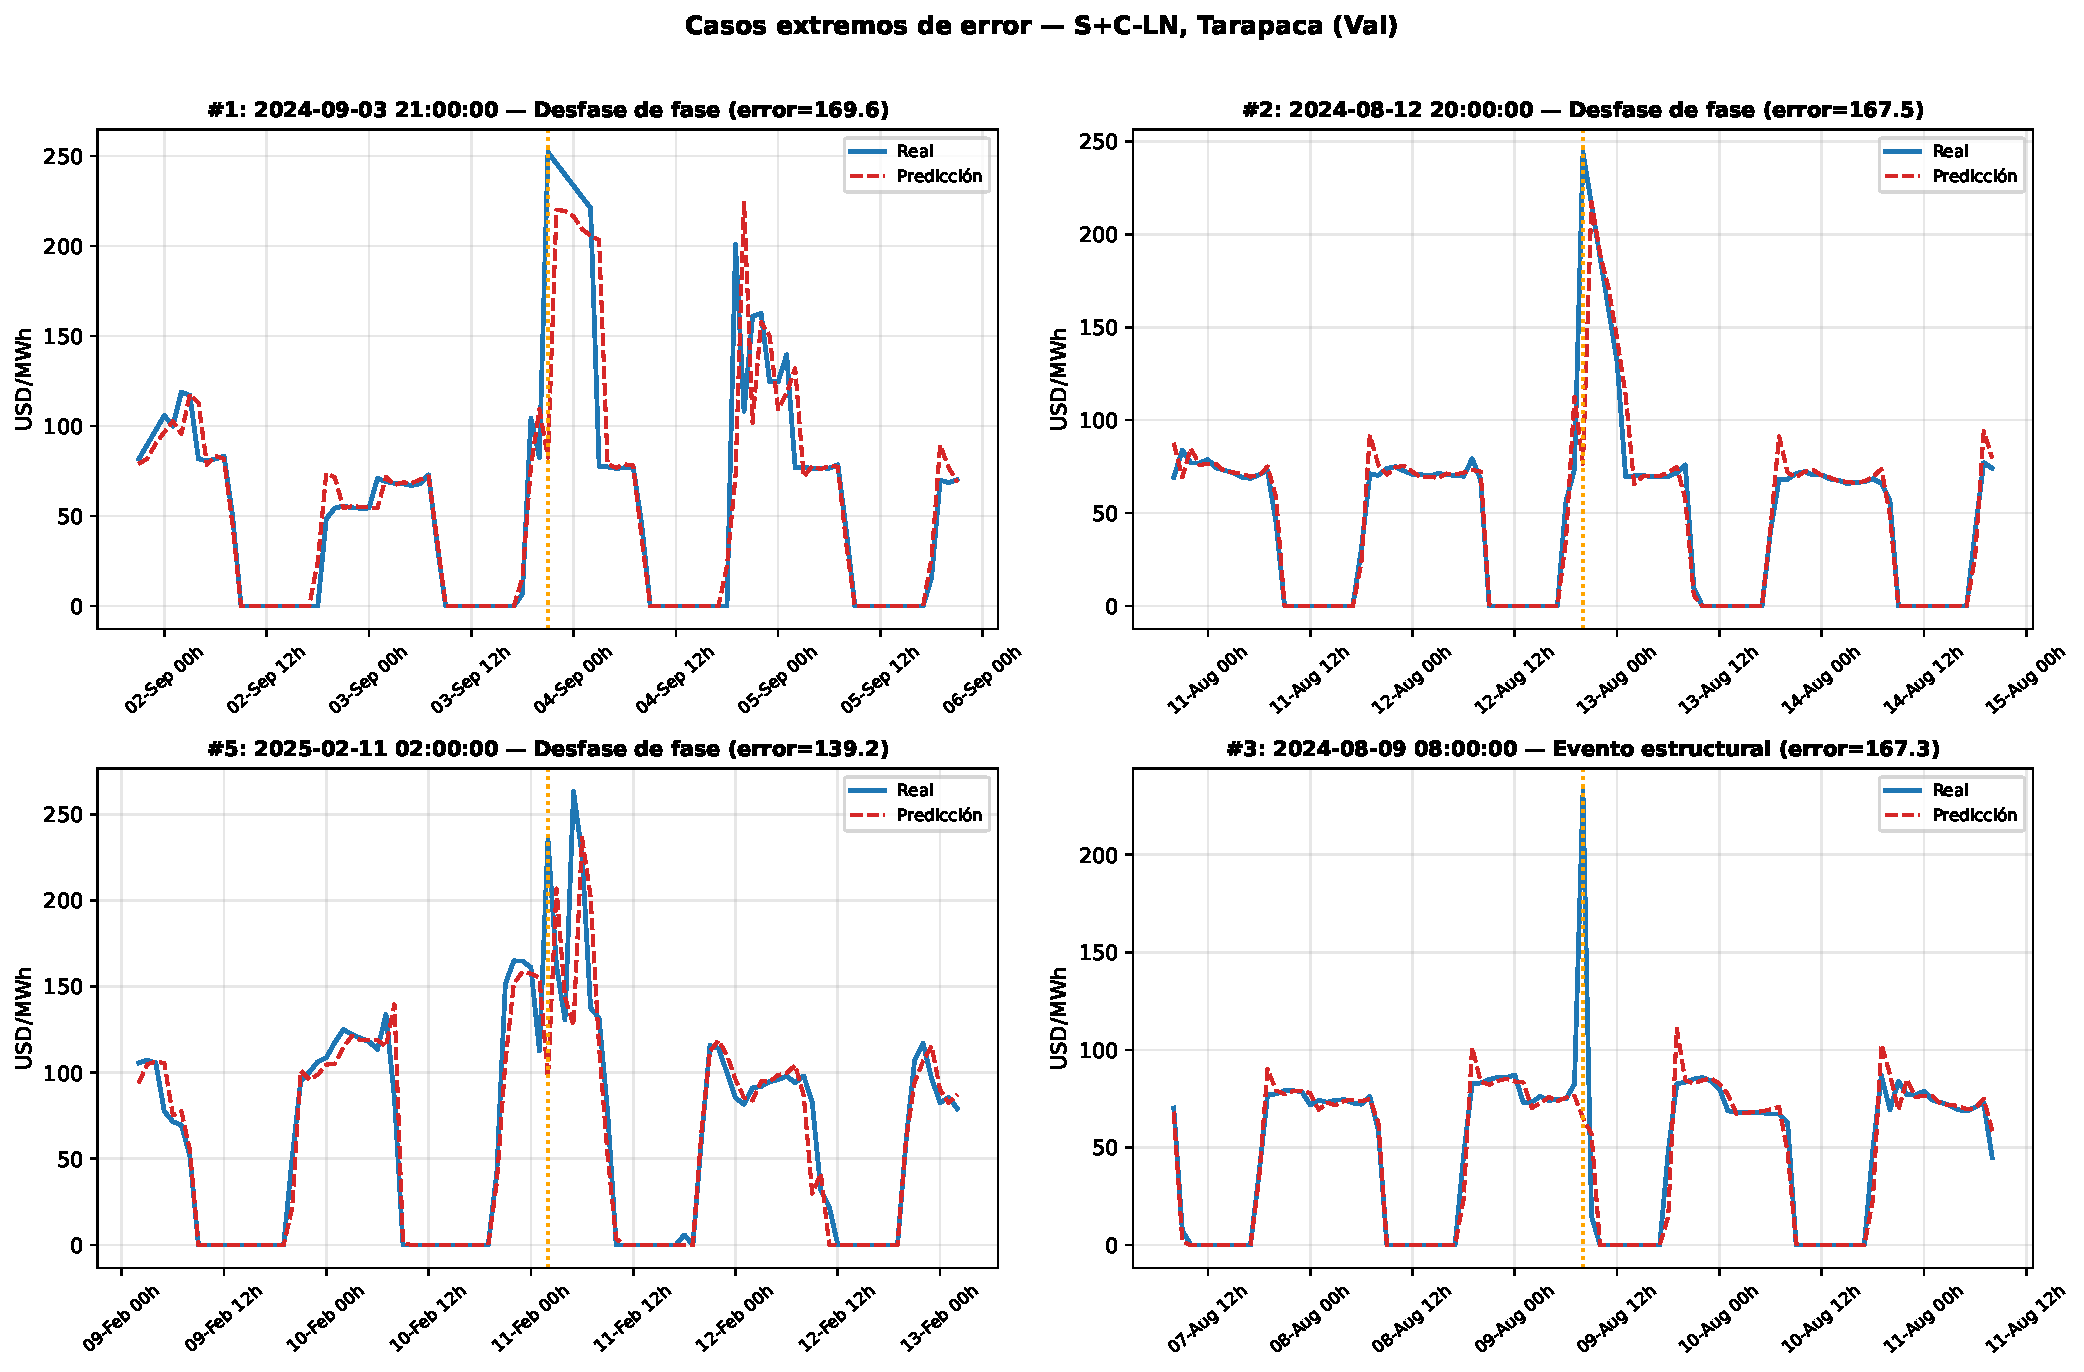
\includegraphics[width=\textwidth]{imagenes/fig_phase_shift_panel_tarapaca.pdf}
    \caption{Casos extremos de error del $\text{TFT}_\text{LN}$ (S+C), Tarapacá.}
    \label{fig:phase_shift_panel_tarapaca}
\end{figure}
